\section{Whirshark}
\label{tool:wireshark}

\subsection*{Pre-capture and Post-capture Processing and Filtering}
see~\ref{network:bpf}

\subsubsection*{Capture Filters}

TO manage the capture filters:
\begin{verbatim}
Menu > Capture > Capture filters\ldots
\end{verbatim}



\begin{figure}
  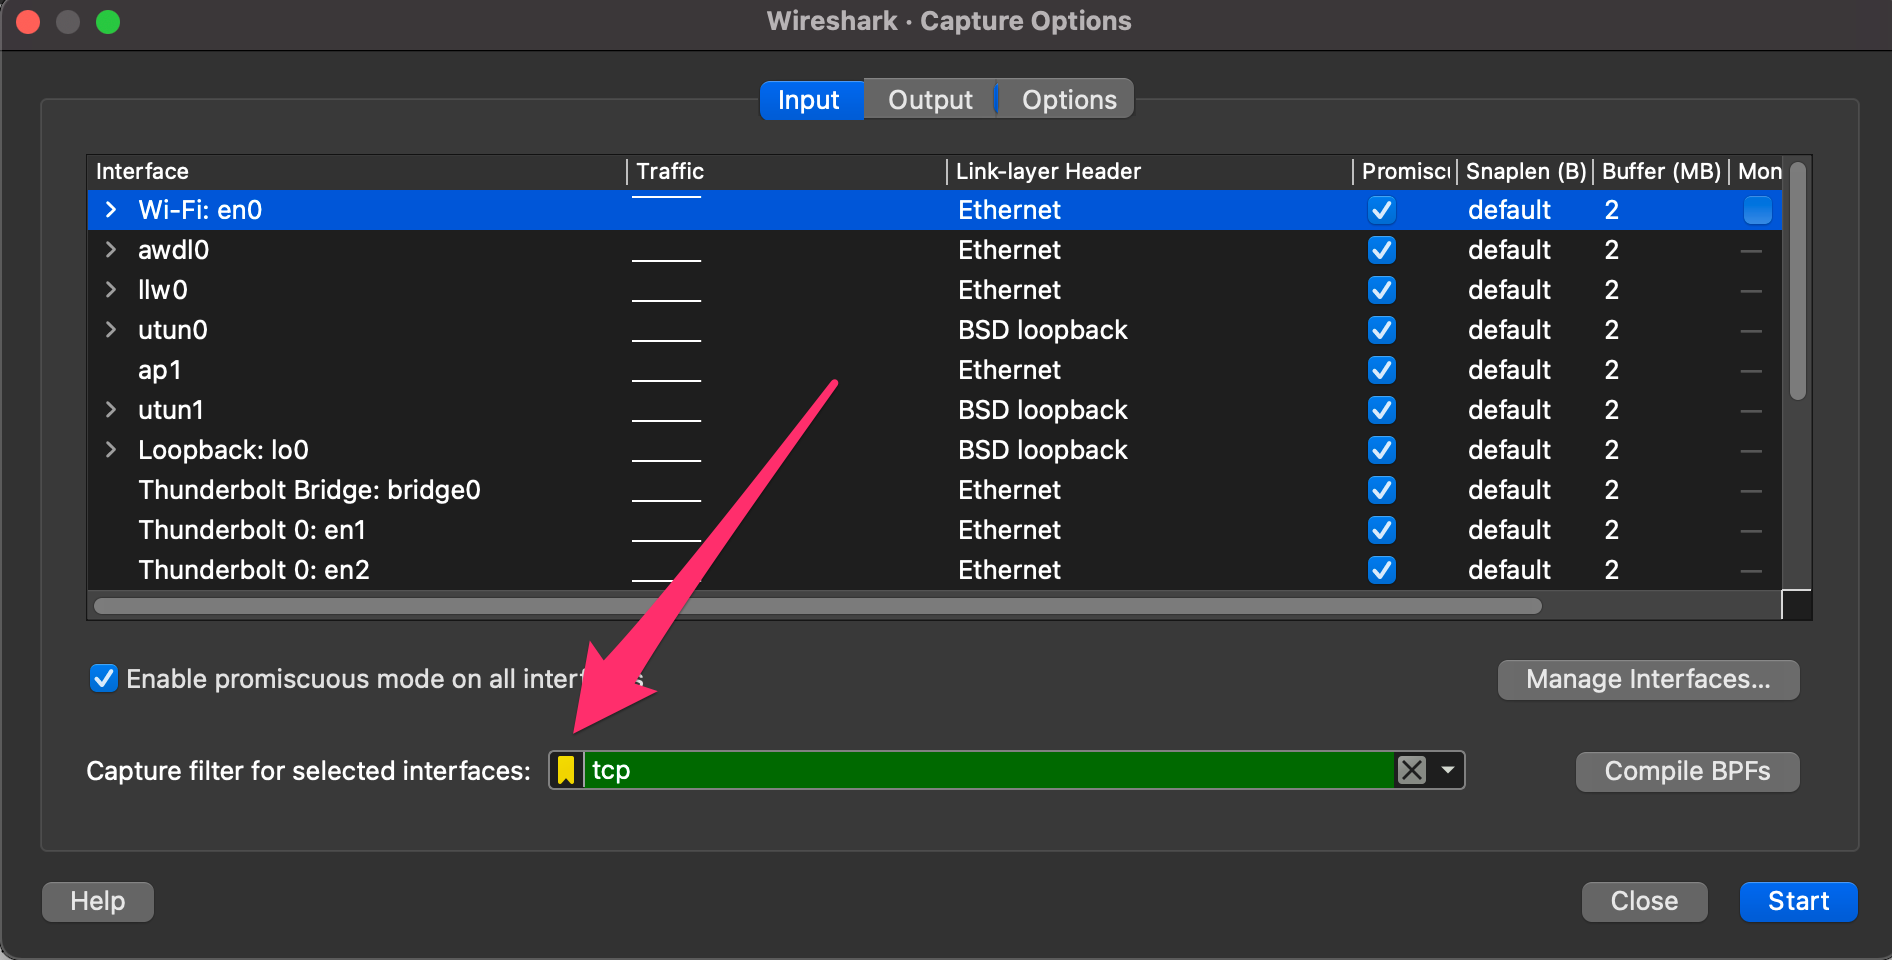
\includegraphics[width=\linewidth]{tools/all/images/wireshark-apply-capture-filter.png}
  \caption{wireshark-apply-capture-filter}
  \label{fig:wireshark-apply-capture-filter}
\end{figure}

\subsubsection*{Display Filters}
TO manage the capture filters:
\begin{verbatim}
Menu > Analyze > Display filters\ldots
\end{verbatim}

\begin{figure}
  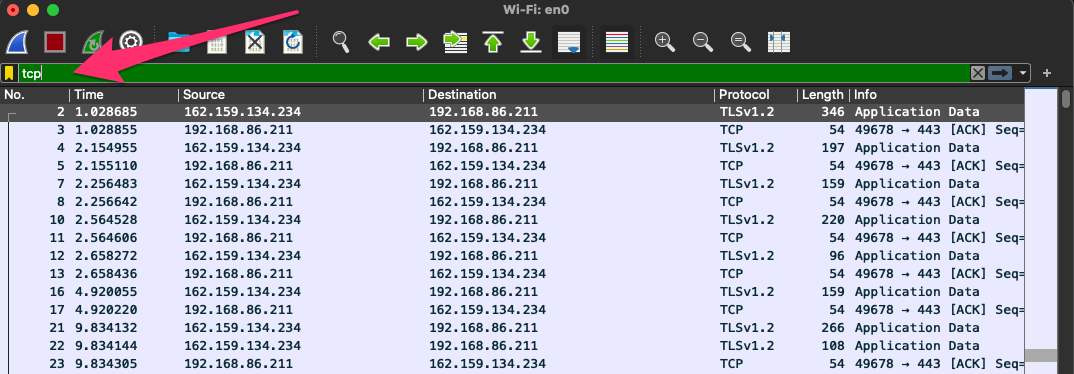
\includegraphics[width=\linewidth]{tools/all/images/wireshark-apply-display-filter.png}
  \caption{wireshark-apply-display-filter}
  \label{fig:wireshark-apply-display-filter}
\end{figure}

\subsection*{Statistics and Analyze}
Provide overview information such as the IP adresses, HTTP requests\ldots

\subsection*{Following streams}

Wireshark can stitch TCP packets back together to recreate the entire stream in a readable format. This ability also allows us to pull data (images, files, etc.) out of the capture. This works for almost any protocol that utilizes TCP as a transport mechanism.

To utilize this feature:
\begin{itemize}
        \item right-click on a packet from the stream we wish to recreate.
        \item select follow → TCP
        \item this will open a new window with the stream stitched back together. From here, we can see the entire conversation.
\end{itemize}

\subsection*{Filter For A Specific TCP Stream}
Set the filter \verb+tcp.stream eq #+ to find and track conversations captured in the pcap file.


\subsection*{Extracting Data and Files From a Capture}
Wireshark can recover many different types of data from streams. It requires to have captured the entire conversation.If we want a more in-depth understanding of how this capability works, check out the Networking 101 Module or research TCP/IP fragmentation.

To extract files from a stream:

\begin{itemize}
        \item stop your capture.
        \item Select the File radial → Export Objects → , then select the protocol format to extract from.
        \item (DICOM, HTTP, SMB, etc.)
\end{itemize}

Another way for example for FTP:
\begin{enumerate}
        \item Identify any FTP traffic using the \verb+ftp+ display filter.
        \item Look at the command controls sent between the server and hosts to
            determine if anything was transferred and who did so with the
            \verb+ftp.request.command+ filter.
        \item Choose a file, then filter for \verb+ftp-data+. Select a packet
            that corresponds with a file of interest and follow the TCP stream
            that correlates to it.
        \item Once done, Change "Show and save data as" to "Raw" and save the content as the original file name.
        \item Validate the extraction by checking the file type.
\end{enumerate}


\subsection*{Provide the key to decrypt the traffic}
\begin{enumerate}
        \item go to Edit → Preferences → Protocols → TLS
        \item On the TLS page, select Edit by RSA keys list → a new window will open.
        \item Click the + to add a new key
        \item Type in the IP address of the server, the port\ldots
        \item Upload the key
\end{enumerate}

\subsection*{Input}
\subsection*{Input}
\subsection*{Input}

\subsection*{links}
\begin{itemize}
    \item \href{https://www.wireshark.org/docs/dfref/}{Display Filter Reference}
\end{itemize}
